\documentclass[../main/main.tex]{subfiles}
\begin{document}

\chapter{Preliminaries}
\section{Quick review of Special Relativity}

Here we expose a quick review of Special Relativity in order to set the notations.

\skipline
Fundamental principles of Special Relativity are followings:
\begin{enumerate}
\item All inertial reference frames are physically equivalent. There is no way to distinguish between different inertial frames in the sense that there is no preferred one. 
\item There exists universal (dimensional) constant: $c\simeq3\times10^8\text{m/s}$, i.e. the speed of massless particles.
\end{enumerate}

\skipline
In order to implement these features basic ingredients are
\begin{enumerate}
\item Space and Time form a unique concept called \textbf{spacetime}. 
\item A spacetime is a collection of points called \textbf{event}.
\item Each inertial frame is associated with a set of \textbf{space time coordinates}. Each events is specified through coordinate system of a fixed initial frame. \[x^\mu=(x^0,x^1,x^2,x^3)\equiv(x^0,x^i)\equiv(ct,x,y,z)\equiv(ct,\vec x)\]
Usually $x,y,z$ are assumed to be Cartesian coordinates.


Given 2 events $A$ and $B$ in  spacetime 




\tikzset{every picture/.style={line width=0.75pt}} %set default line width to 0.75pt     
\[
\begin{tikzpicture}[x=0.75pt,y=0.75pt,yscale=-1,xscale=1]
%uncomment if require: \path (0,300); %set diagram left start at 0, and has height of 300

%Straight Lines [id:da9013720818372855] 
\draw    (195,224) -- (195,141) ;
\draw [shift={(195,139)}, rotate = 450] [color={rgb, 255:red, 0; green, 0; blue, 0 }  ][line width=0.75]    (10.93,-3.29) .. controls (6.95,-1.4) and (3.31,-0.3) .. (0,0) .. controls (3.31,0.3) and (6.95,1.4) .. (10.93,3.29)   ;
%Straight Lines [id:da7261382621997787] 
\draw    (195,224) -- (302.5,224) ;
\draw [shift={(304.5,224)}, rotate = 180] [color={rgb, 255:red, 0; green, 0; blue, 0 }  ][line width=0.75]    (10.93,-3.29) .. controls (6.95,-1.4) and (3.31,-0.3) .. (0,0) .. controls (3.31,0.3) and (6.95,1.4) .. (10.93,3.29)   ;
%Straight Lines [id:da22577623387415535] 
\draw    (195,224) -- (141.99,271.66) ;
\draw [shift={(140.5,273)}, rotate = 318.03999999999996] [color={rgb, 255:red, 0; green, 0; blue, 0 }  ][line width=0.75]    (10.93,-3.29) .. controls (6.95,-1.4) and (3.31,-0.3) .. (0,0) .. controls (3.31,0.3) and (6.95,1.4) .. (10.93,3.29)   ;
%Straight Lines [id:da04380450147553239] 
\draw [color={rgb, 255:red, 65; green, 117; blue, 5 }  ,draw opacity=1 ][line width=0.75]    (219.5,203) -- (276.5,169) ;
\draw [shift={(276.5,169)}, rotate = 329.18] [color={rgb, 255:red, 65; green, 117; blue, 5 }  ,draw opacity=1 ][fill={rgb, 255:red, 65; green, 117; blue, 5 }  ,fill opacity=1 ][line width=0.75]      (0, 0) circle [x radius= 1.9, y radius= 1.9]   ;
\draw [shift={(219.5,203)}, rotate = 329.18] [color={rgb, 255:red, 65; green, 117; blue, 5 }  ,draw opacity=1 ][fill={rgb, 255:red, 65; green, 117; blue, 5 }  ,fill opacity=1 ][line width=0.75]      (0, 0) circle [x radius= 1.5, y radius= 1.5]   ;

% Text Node
\draw (120,137) node    {$$};
% Text Node
\draw (283,258) node    {$x,y,z$};
% Text Node
\draw (177,141) node    {$ct$};
% Text Node
\draw (210,207) node    {$A$};
% Text Node
\draw (280,157) node    {$B$};


\end{tikzpicture}\]

their distance is $\Delta x^\mu=x^\mu_B-x_A^\mu$. We introduce the (squared) \textbf{Minkowski distance}
\[\Delta s^2=\eta_{\mu\nu}\Delta x^\mu\Delta^\nu\quad\text{where}\quad\eta_{\mu\nu}=\begin{pmatrix}-1&&&\\&1&&\\&&1&\\&&&1\end{pmatrix}\]
where $\eta_{\mu\nu}$ is \textbf{Minkowski metric}.
This induces the \textbf{line element}
\[\de s^2=\eta_{\mu\nu}\de x^\mu\de x^\nu\]
This element is scalar quantity and therefore does not depends on the specific inertial frame.

The quantity $\Delta s^2$ has an intrinsic meaning
\[\begin{cases}\begin{alignedat}{2}
&\Delta s^2>0\quad&&:\quad \Delta x^\mu\text{ is \textbf{space-like} vector}\\
&\Delta s^2=0\quad&&:\quad \Delta x^\mu\text{ is \textbf{time-like} vector}\\
&\Delta s^2<0\quad&&:\quad \Delta x^\mu\text{ is \textbf{light-like/null} vector}
\end{alignedat}\end{cases}\]
Space-like vector means that exists different frames were two events are simultaneous. Time-like vector means that exists different frames where two events have same space coordinates but they happen at different times. Light-like vectors means that two events may be connected by a light signal.

\item Allowed transformations for spacetime vectors must preserve the line element: $\Delta\tilde s^2=\Delta s^2$. These transformations are the \textbf{Poincaré Transformations}

\[x^\mu\quad\to\quad\tilde x^\mu={\Lambda^\mu}_\nu x^\nu+a^\mu\qquad\text{with}\qquad{\Lambda^\rho}_\mu{\Lambda^\sigma}_\nu\eta_{\rho\sigma}=\eta_{\mu\nu}\]


\end{enumerate}

\skipline
Once we have reformulated notions of space and time, we have to reformulate law of physics in such a way they does not depends on the reference frame.

Trajectories of point like-particles are associated to curved \textbf{wordlines} in space time and described evolution of events. Mathematically they are described by maps from $\RR$ into a set of four functions: $\lambda\in\RR\to x^\mu(\lambda)$. Near if we consider nearby events separated by infinitesimal shift we can obtain infinitesimal variation of coordinates:
\[\de x^\mu(\lambda)\equiv x^\mu(\lambda+\de\lambda)-x^\mu(\lambda)=\frac{\de x^\mu(\lambda)}{\de\lambda}\de\lambda\]
Since no particles can move at a speed higher then light this implies that $\de s^2$ must be time-like. Notice that choice of parameter $\lambda$ is free. One possible choice of this parameter is the \textbf{(differential) proper time}:
\begin{align*}
\de\tau\equiv\sqrt{-\de s^2}
&=\de\lambda\sqrt{-\eta_{\mu\nu}\dot x^\mu(\lambda)\dot x^\nu(\lambda)}
=c\,\de t\sqrt{1-\frac{v^2}{c^2}}\equiv\frac{c\,\de t}\gamma
\end{align*}
where third step holds if $\lambda\equiv t$. If we define $\beta\equiv v/c$ \footnote{This is the speed in natural units, i.e. in units of $\beta$. If we set $c=1$ then $v=\beta$.}, then $\gamma=1/\sqrt{1-\beta^2}$ is called \textbf{Lorentz factor}. Notice that last step implies time dilatation at higher velocities. For $\lambda=t$ we obtain
\[\tau=c\int\de t\sqrt{1-\frac{v^2}{c^2}}\]
i.e. with this definition the proper time has dimension of a length $[\tau]=L$. Physically the proper times it's the time measured by a clock moving along the trajectory. 

Proper time allow us to define a vector called \textbf{4-velocity} that can be identified as relativistig generalization of velocity. Namely:
\[u^\mu(\tau)=\frac{\de x^\mu(\tau)}{\de\tau}=\left(\gamma,\gamma\frac{\vec v}{c}\right)\]
Notice 
\[u^\mu u_\mu=-1\]
i.e. is a time-like vector. Moreover, this vector has only three degrees of freedom, since one component is fixed by previous propriety.


Now we can define the generalization of acceleration, \textbf{4-acceleration}, as follows
\[\alpha^\mu(\tau)=\frac{\de u^\mu(\tau)}{\de \tau}\]
Notice that, as we expected, 4-acceleration is orthogonal to 4-velocity
\[u_\mu\alpha^\mu=0\]
and this implies that $\alpha^\mu$ is a space-like since it is orthogonal to a time-like vector.

This proves a relativistic generalization of distance, speed and acceleration. Also laws of dynamic can be generalizated, in particular if we define the \textbf{four-force} $f^\mu$ as the generalization of force we can obtain the
 \textbf{Relativistic Second Newton's law}:
\[mc\alpha^\mu\equiv\frac{\de p^\mu}{\de\tau}=f^\mu\]
where we used four acceleration or equivalently the generalization of newtonian momentum, \textbf{4-momentum},
\[p^\mu\equiv mcu^\mu=\p{\frac Ec,\vec p}\]

For example, for Lorentz force
\[\vec F_L=e\p{\vec E+\frac1c\vec v\cross\vec B}\]
can be generalizzated in a manifestly covariant way into\footnote{Here is evident that this formula does not change under Poincaré transformations.}
\[f^\mu_L=\frac ecF^{\mu\nu}u_\nu\hspace{1.5cm}\text{with}\quad F^{\mu\nu}=
\begin{pmatrix}0&E_1&E_2&E_3\\-E_1&0&B_3&-B_2\\-E_2&-B_3&0&B_1\\-E_3&B_2&-B_1&0\end{pmatrix}\]
where $F^{\mu\nu}$ is the \textbf{EM-Tensor}.

We can also rewrite Maxwell equations into two covariant equation
\[\partial_\mu F^{\mu\nu}=-\frac{4\pi}{c}j^\nu\quad,\quad\partial_{[\mu}F_{\nu\rho]}=0\]
where the former, inhomogeneous, shows the \textbf{4-current} $j^\mu=(c\rho, \vec j)$. The second equation, homogeneous, exhibits total antisymmetrized indexes\footnote{$\partial_{[\mu}F_{\nu\rho]}=\partial_{\mu}F_{\nu\rho}+\partial_\rho F_{\mu\nu}+\partial_\nu F_{\rho\mu}$.}. Each of these equations contains 2 independent equations.


We can conclude saying that all possible interactions can be written in a covariant way, except from gravitation. In order to include this force General Relativity has been developed.


%%%%%%%%%%%%%%%%%%%%%%%%%%%%%%%%%%%


\section{Relativity and Gravitation}

Before Einstein formulated General Relativity the accepted theory for Gravity was Newton's one.

In Newton theories particles interact according to \textbf{Newton's universal gravity law}:
\[\vec F_G=-\frac{GmM}{\vert\Delta\vec r\vert^3}\Delta\vec r\qquad G\simeq6.67\times10^{-11} \frac{m^3}{kg\cdot s^2} \]
where $\vec F_G$ is the (always) attractive gravitational force, $\Delta\vec r$ is the distance (at same time) between particles, and $G$ is \textbf{Newton's gravitational constant}.

The point is that this law is not invariant under Poincaré. Practically this is evident since positions are evaluated at a certain time and therefore when a particle moves the corresponding formula for gravitational force changes instantaneously. This is unphysical since physical signal cannot travel with a velocity higher than  speed of light. This instantaneous interaction between particles cannot be compatible with special relativity.

One possible strategy to way out is to look at an analogy with Coulomb force between two particles $A$ and $B$:
\[\vec F_C=e_B\vec E=\frac{e_Be_A}{\vert\Delta\vec r\vert^3}\Delta\vec r\]
These formulas are very analogous. The coulomb force is valid only in a static setting in which one put one particle in the electric field of the other. When particles moves this particles does not hold anymore since we have to consider magnetic field and Coulomb force must be substituted with the more general Lorentz force.


Let's go further with the analogy. In gravity we can introduce a potential which is completely analogous to electric static potential:
\begin{align*}
\nabla^2\Phi=4\pi G\rho_M\hspace{2cm}G\rho_M\leftrightarrow&-\rho_{el}\hspace{2cm}\nabla^2\Phi_{el}=-\vect\nabla\cdot\vec E=-4\pi\rho_{el}\\
\vec F_G=-m\vect\nabla\Phi\hspace{2.8cm}m\leftrightarrow&e\hspace{3.2cm}\vec F_C=e\vec E=-e\vect\nabla\Phi_{el}
\end{align*}
where $\Phi$ describe potentials and $\rho$ describes distributions. 

In order to make Coulomb force compatible with special relativity we have to consider EM theory in a wider way, in order to express quantities in tensorial way:
\begin{alignat*}{2}
&\Phi_{el}\hspace{1cm}&&\rightarrow\quad	A^\mu=(\Phi, \vec A)\\
&\vec E\hspace{1cm}&&\rightarrow\quad	F_{\mu\nu}=\partial_\mu A_\nu-\partial_\nu A_\mu\\
&\rho_{el}\hspace{1cm}&&\rightarrow\quad	j^\mu=(c\rho_{el},\vec j)\\
m\vec a&=\vec F_c\hspace{1cm}&&\rightarrow\quad	mc\alpha^\mu=f^\mu_L=\frac ecF^{\mu\nu}u_\nu
\end{alignat*}
So in order to understand how to make gravity compatible with spacial relativity we should find gravitational analogous to previous completions of Coulomb theory. We will start from the last  step, i.e. we have to understand what happen when we put a particle in an external gravitational field and then derive covariant relations, which in non relativistic approximation must leads to Newton's law
\[m\vec a=\vec F_G\]
In particular we have to find which is relativistic generalization of gravitational field $\Phi_G$ that allows us to build a covariant theory of gravitation.

\skipline
First of all we have to highlight a deep difference between $\vec F_G$ and $\vec F_C$ that in principle we should distinguish between two forces. For gravitational theory the force is proportional to the mass of the particle, while for Coulomb law the force is proportional to the charge. In order to make the analogy precise we have should distinguish between two different concepts of mass, that in principle may be differnet\footnote{For the moment we consider the non-relativistic limit}
\begin{alignat*}{2}
&\text{\textbf{interial mass }} m_I\quad&&:\quad m_I\vec a=\vec F_G\\
&\text{\textbf{gravitational mass }} m_G\quad&&:\quad\vec F_G=-m_G\vect\nabla\cdot\Phi\hspace{1cm}m_G\sim\text{gravitational charge}
\end{alignat*}
the fact that in Newton's law $m_G\equiv m_I$ is an highly not-obvious feature from theoretical point of view. Indeed, this is the Newtonian manifestation of the \textbf{(Weak) Equivalence principle}.

\subsection{The Equivalence principle}

The Equivalence principle is the consequence of the central observation that $m_G\equiv m_I$. This implies that
\[\slashed m_I\vec a=\vec F_G=-\slashed m_G\vect\nabla\Phi\quad\Rightarrow\quad\boxed{\vec a=-\vect\nabla\Phi}\]
i.e. acceleration of a mass is the same for each value of $m$ (for example this does not happen for Coulomb interaction, where acceleration depends on the charge of the particle). Then for the same field $\Phi$ all bodies fall with the same acceleration. 

This is a very important observation: if $\vect\nabla\Phi$ is considered approximatively constant in a chosen frame, then we cannot distinguish between gravitational force and an apparent force due to an acceleration in the opposite direction of this frame with respect to an inertial frame. 


\begin{figure}[H]
\centering
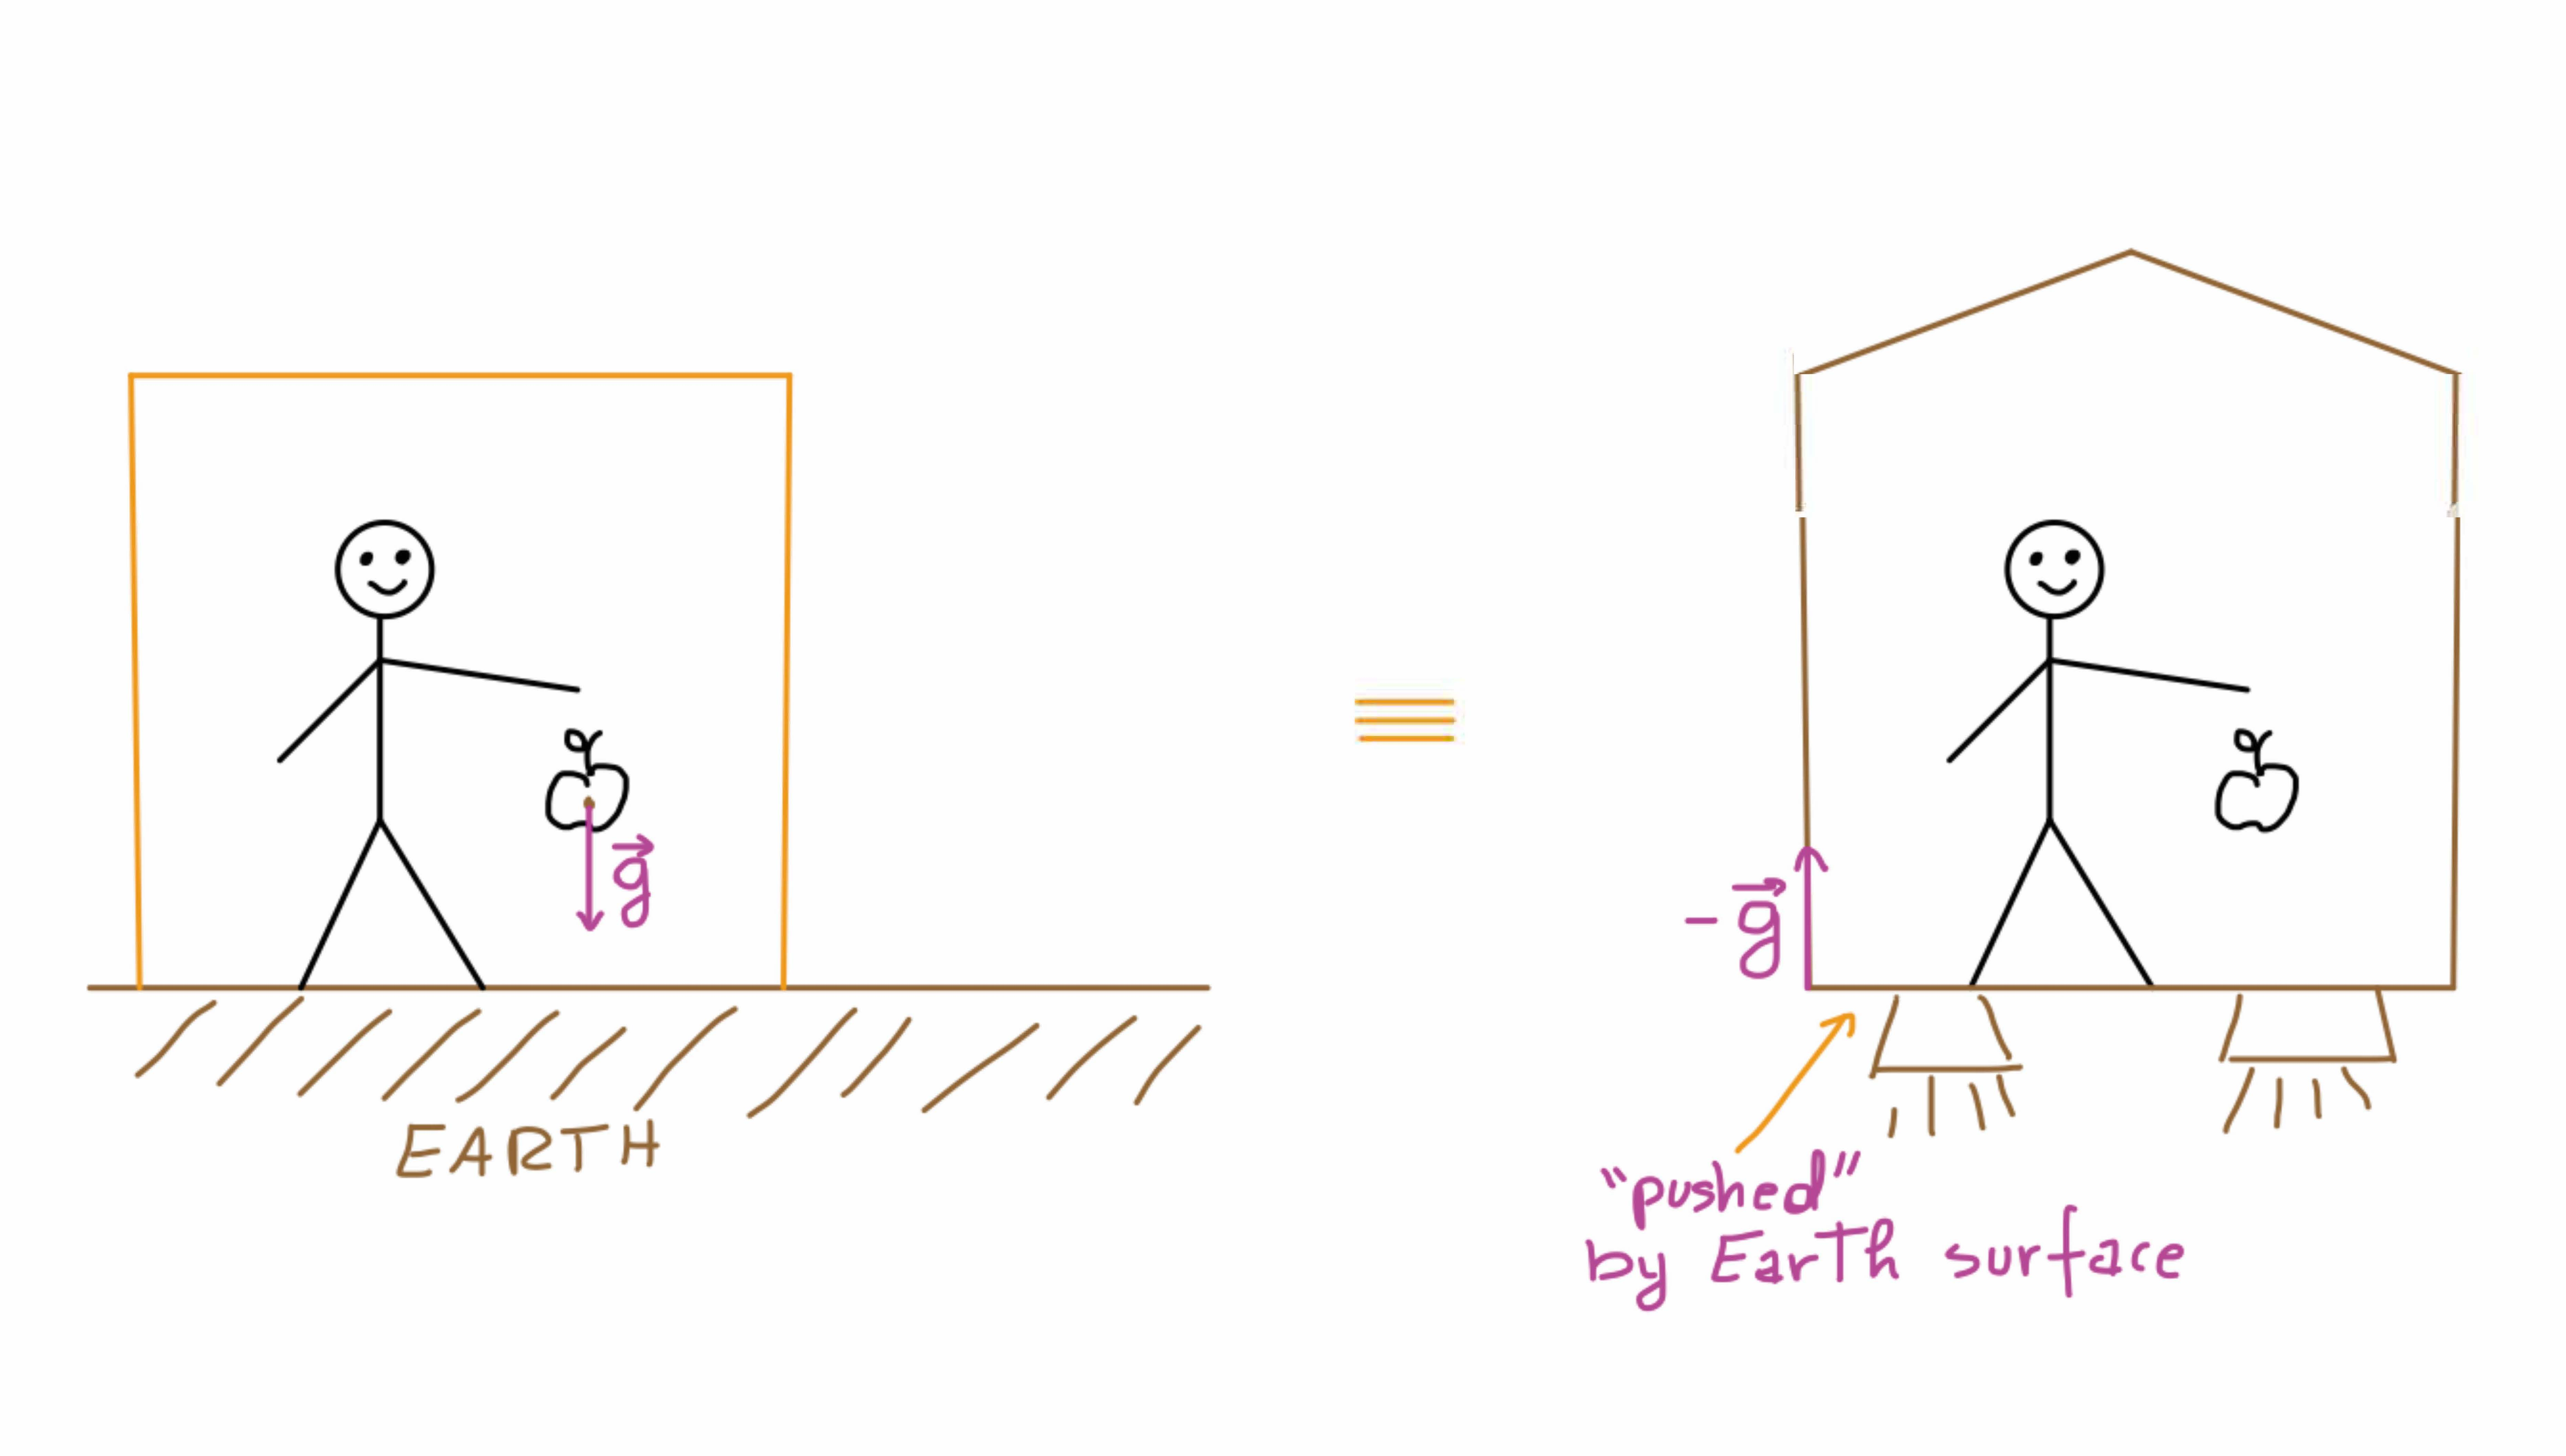
\includegraphics[width=11cm]{../img/equivalence-principle.jpg}
\caption{In the first figure the apple falls down, while in the second the rocket moves upward. Our Rocket Man can't fell any difference.}
\end{figure}

\subsubsection{``The happiest thought of Einstein life'':}
\begin{mdframed}[style=mybox]
``The gravitational field has only a \emph{relative} existence $\dots$ because for an observer freely falling from the roof of a house there exists - at least in the immediate surroundings - no gravitation''
\end{mdframed}

In other words, a freely falling system can be identified (up to some approximations) to an ``inertial'' frame\footnote{We will have to specify this concept in formalization of General Relativity.} in the sense that within a freely falling system there is no way to distinguish between these two situations. 

This leads to the formulation of \textbf{(Einstein) Equivalence ``Principle''} (\textbf{EEP})
\begin{mdframed}[style=mybox]
In a small enough region of spacetime, the laws of physics reduce to those of Special Relativity: it is impossible to detect the existence of a gravitational field by means of local experiments.
\end{mdframed}

In other words though local experiments it is impossible to distinguish between a system accelerated and a system subjected to gravitational field.
The caveat ``small enough'' refers to the \emph{Tidal effects}, i.e. the previous statement holds only if the gravitational field can be considerated uniform and constant. Let $l$ be the typical length scale of our experiment and $L$ be the distance from the mass that origins the gravitational field, then ``small enough'' means
\[\p{\frac lL}^n\ll1\]

\begin{figure}[H]
\centering
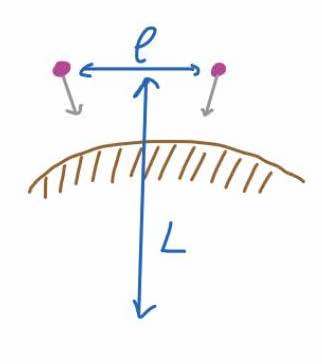
\includegraphics[width=4cm]{../img/Tidal-effect.jpg}
\caption{Tidal effect}
\end{figure}

There are 3 kinds of equivalence principles:\footnote{In the paper \emph{Di Casola, Liberati \& Sonego}, 1310.7426, are described differences of these statements and experiments evidence for each principle.}
\begin{enumerate}
\item\textbf{Weak Equivalence Principle (WEP)}: regards only experiments on freely falling non back-reacting test particles (direct consequence of $m_G=m_I$.
\item\textbf{Einstein Equivalence Principle (EEP)}: previously stated, include also other non-gravitational local experiments (no backreaction)
\item\textbf{Strong Equivalence Principle (SEP)}: includes also local gravitational effects (includes gravitational effects, i.e. back-reaction). For instance it consider also inertial masses in experiments involving them variation measure when accelerated. 
\end{enumerate}

One can think about these principles as heuristic ideas, which will be defined in a more precise way by General Relativity in a concrete framework. 


There are some immediate implications of these principles. First \emph{light is deflected} in presence of gravitation potential, this is obvious watching at the next image


\begin{figure}[H]
\centering
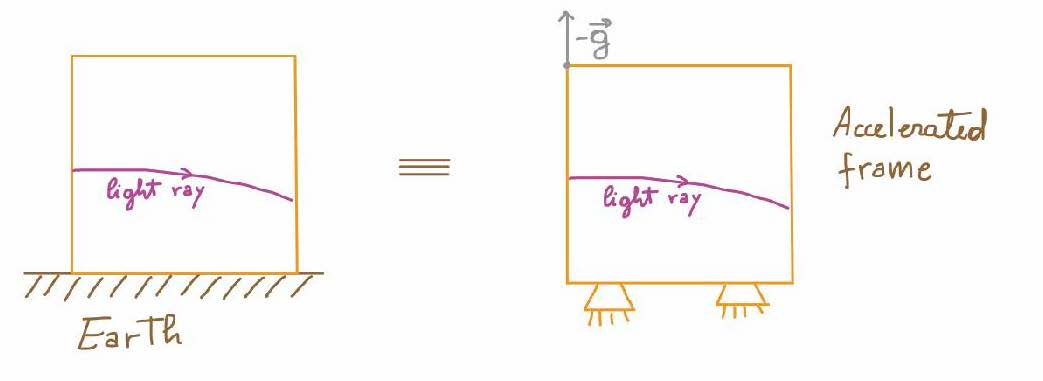
\includegraphics[width=11cm]{../img/light-deflection.jpg}
\end{figure}

Then, we will see \emph{gravitational time dilatation and red-shift of light}:

\begin{figure}[H]
\centering
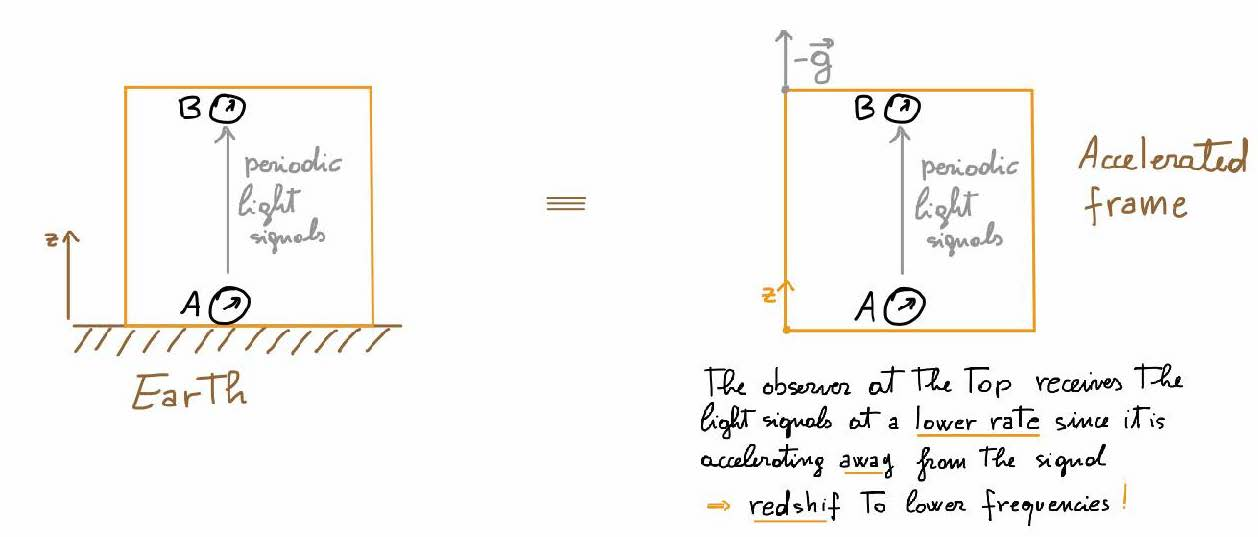
\includegraphics[width=11.5cm]{../img/redshift.jpg}
\end{figure}

The second frame is accelerated, then during the interval which the light signal need to go from a clock A to the clock B the clock B gets some additional velocity, so frequency measured by B is lower than the frequency measured by A:
\[v_B-v_a\simeq g\Delta t=g\frac{\Delta z}{c}\]
and we can observe a \emph{Doppler effect} 
\[\frac{\nu_B-\nu_A}{\nu_a}\simeq\frac{v_A-v_B}{c}=\frac{g(z_A-z_B)}{c^2}\]
If we take $\Phi\simeq gz$ we can obtain an explicit relation between redshift and acceleration
\[\frac{\nu_B-\nu_A}{\nu_A}\simeq\frac1{c^2}(\Phi_A-\Phi_B)<0\]
Viceversa, since frequency is the inverse of time interval, this can be interpreted as a time dilatation.
In other words, we can see that clock B ``sees'' clock A moving more slowly.\footnote{See Hartle's book for the discussion of Redshift using time dilatation instead of moving clocks.}














\end{document}